\documentclass[titlepage]{article}
\usepackage{babel}
\usepackage{amsmath}
\usepackage{amssymb}
\usepackage{amsthm}
\usepackage{multicol} %spalten in seite
\usepackage{graphicx} %bilder einfügen
\usepackage{tabto} %tabulator mit \tab
\usepackage{hyperref}
\usepackage{xcolor}
\usepackage[T1]{fontenc}
\usepackage[utf8]{inputenc}
\usepackage{listings} %quellcode
\pagestyle{plain}
\pagenumbering{arabic}
\renewcommand{\arraystretch}{1.3} %vertikaler abstand von tabellen
\newcommand{\n}{\newline}
\usepackage[left=20mm, right=15mm, top=25mm, bottom=30mm, paper=a4paper]{geometry}

\usepackage{pgfplots}
\pgfplotsset{compat=1.15}
\usepackage{mathrsfs}
\usetikzlibrary{arrows}
\pagestyle{empty}

\lstset{ 
	backgroundcolor=\color{white},   % choose the background color; you must add \usepackage{color} or \usepackage{xcolor}; should come as last argument
	basicstyle=\footnotesize,        % the size of the fonts that are used for the code
	breakatwhitespace=false,         % sets if automatic breaks should only happen at whitespace
	breaklines=true,                 % sets automatic line breaking
	captionpos=b,                    % sets the caption-position to bottom
	commentstyle=\color{mygreen},    % comment style
	deletekeywords={...},            % if you want to delete keywords from the given language
	escapeinside={\%*}{*)},          % if you want to add LaTeX within your code
	extendedchars=true,              % lets you use non-ASCII characters; for 8-bits encodings only, does not work with UTF-8
	firstnumber=1,                % start line enumeration with line 1000
	%frame=single,	                   % adds a frame around the code
	keepspaces=true,                 % keeps spaces in text, useful for keeping indentation of code (possibly needs columns=flexible)
	keywordstyle=\color{blue},       % keyword style
	language=Octave,                 % the language of the code
	morekeywords={*,...},            % if you want to add more keywords to the set
	numbers=left,                    % where to put the line-numbers; possible values are (none, left, right)
	numbersep=5pt,                   % how far the line-numbers are from the code
	numberstyle=\tiny\color{mygray}, % the style that is used for the line-numbers
	rulecolor=\color{black},         % if not set, the frame-color may be changed on line-breaks within not-black text (e.g. comments (green here))
	showspaces=false,                % show spaces everywhere adding particular underscores; it overrides 'showstringspaces'
	showstringspaces=false,          % underline spaces within strings only
	showtabs=false,                  % show tabs within strings adding particular underscores
	stepnumber=1,                    % the step between two line-numbers. If it's 1, each line will be numbered
	stringstyle=\color{mymauve},     % string literal style
	tabsize=2,	                   % sets default tabsize to 2 spaces
	title=\lstname                   % show the filename of files included with \lstinputlisting; also try caption instead of title
}

\begin{document}
	
	\title{Diskrete Strukturen - Übung 02}
	\author{Felix Tischler, Martrikelnummer: 191498}
	\date{\today}
	\maketitle
	
	\section*{1.) Turm von Hanoi}
		\subsection*{a)}
		A := Startstapel, B:= Hilfsstapel, C:= Zielstapel. In der unten aufgeführten Tabelle wird verkürzt "AC" oder eine andere beliebige Abfolge von Buchstaben verwendet. Wobei "AC" steht für "Bewege die oberste Scheibe von A nach C". Es wird logischerweise immer die aktuell oberste Scheibe bewegt und der Buchstabe gibt an um auf zwischen welchen Stapeln die Scheibe bewegt wird.
		
		\definecolor{ududff}{rgb}{0.30196078431372547,0.30196078431372547,1}
		\begin{tikzpicture}[line cap=round,line join=round,>=triangle 45,x=1cm,y=1cm]
			\clip(-8.178128586445613,-2.498131578998504) rectangle (8.742545996854185,5.741884429014671);
			\draw [line width=2pt] (-6,1)-- (-3,1);
			\draw [line width=2pt] (-2,1)-- (1,1);
			\draw [line width=2pt] (2,1)-- (5,1);
			\draw [line width=2pt] (-4.5,1)-- (-4.5,3);
			\draw [line width=2pt] (-0.5,1)-- (-0.5,3);
			\draw [line width=2pt] (3.5,1)-- (3.5,3);
			\begin{scriptsize}
				\draw[color=ududff] (-4.520795278076125,0.5177037397340701) node {\LARGE$A$};
				\draw[color=ududff] (-0.4668836591605484,0.5066876755522343) node {\LARGE$B$};
				\draw[color=ududff] (3.4768673179366707,0.5617679964614133) node {\LARGE$C$};
			\end{scriptsize}
		\end{tikzpicture}
	
		\definecolor{ududff}{rgb}{0.30196078431372547,0.30196078431372547,1}
		\begin{tikzpicture}[line cap=round,line join=round,>=triangle 45,x=1cm,y=1cm]
			\clip(-8.214444482965344,-2.323934393114055) rectangle (7.591606116270004,5.3732829559927415);
			\draw [line width=2pt] (-6,1)-- (-3,1);
			\draw [line width=2pt] (-2,1)-- (1,1);
			\draw [line width=2pt] (2,1)-- (5,1);
			\draw [line width=2pt] (-4.5,1)-- (-4.5,3);
			\draw [line width=2pt] (-0.5,1)-- (-0.5,3);
			\draw [line width=2pt] (3.5,1)-- (3.5,3);
			\draw [rotate around={-0.6138598631093254:(-4.448158988616272,1.3137211321656939)},line width=2pt] (-4.448158988616272,1.3137211321656939) ellipse (1.446392475951558cm and 0.12776628927858438cm);
			\draw [rotate around={-0.8145770497597213:(-4.412142597276715,1.643013852983095)},line width=2pt] (-4.412142597276715,1.643013852983095) ellipse (1.088550658656826cm and 0.07808146788934615cm);
			\draw [rotate around={-1.4232048466331035:(-4.443013789853496,1.9877421700888152)},line width=2pt] (-4.443013789853496,1.9877421700888152) ellipse (0.8326080241409952cm and 0.0812655971125414cm);
			\begin{scriptsize}
				\draw[color=ududff] (-4.5304821688206465,0.59405605712573) node {\LARGE$A$};
				\draw[color=ududff] (-0.47606554375637156,0.5837656596001863) node {\LARGE$B$};
				\draw[color=ududff] (3.4651567085269215,0.5352176472279055) node {\LARGE$C$};
			\end{scriptsize}
		\end{tikzpicture}
			\begin{table}[h]
				\begin{tabular}{l|llllllllllllllll}
					n&&&&&&&&&&&&&&&&\\
					1&AC&&&&&&&&&&&&&&&\\
					2&AB&AC&BC&&&&&&&&&&&&&\\
					3&AC&AB&CB&AC&BA&BC&AC&&&&&&&&&\\
					4&AB&AC&BC&AB&CA&CB&AB&AC&BC&BA&CA&BC&AB&AC&BC&\\\hline
					5&AC&AB&CB&AC&BA&BC&AC&AB&CB&CA&BA&CB&AC&AB&CB&\\
					&AC&BA&BC&AC&BA&CB&CA&BA&BC&AC&AB&CB&AC&BA&BC&AC
				\end{tabular}
			\end{table}
			\subsection*{b)}
			Wenn man sich an einem Beispiel von \textcolor{blue}{n = 4} überlegt wie genau man die Scheiben bewegen muss, dann wird relativ schnell klar, dass man zunächst \textcolor{red}{3} Scheiben also \textcolor{red}{n-1} auf den Hilfsstapel (B) bewegen muss, und zwar genau diejenigen welche über der größten Scheibe liegen. Die Verschiebung erfolgt in T(\textcolor{red}{n-1}) also T(\textcolor{red}{2+1})=T(\textcolor{red}{3}) Schritten. Anschließend muss die Größte Scheibe auf den Zielstapel (C) gelegt werden dies verbraucht exakt \textcolor{orange}{\textbf{1}} Zug. Nun sind noch \textcolor{red}{3} (\textcolor{red}{n-1}) Scheiben auf den Zielstapel (C) zu legen. Dies verbraucht erneut T(\textcolor{red}{3}) Schritte. Es muss sich hierbei um die \textit{kleinstmögliche} Anzahl handel, da die Regel (H2) uns zwingt immer die größte Scheibe als erstes zu bewegen, somit muss man zunächst alle darüber (\textcolor{red}{n-1},) weg bewegen, dann die größte Scheibe \textcolor{orange}{\textbf{1}} mal bewegen und anschließend wieder die ursprünglich drauf liegenden Scheiben (\textcolor{red}{n-1}) erneut auf die größte Scheibe legen. Somit verschiebt man 2 mal \textcolor{red}{n-1} Scheiben und \textcolor{orange}{\textbf{1}} mal die Größte. Wenn man nun Anstelle von \textcolor{blue}{n = 4} einfach \textcolor{blue}{n+1 = 4} schreibt und somit statt \textcolor{red}{n-1 = 3} einfach \textcolor{red}{n = 3}, dann ergeben sich folgende Zusammenhänge:
			\begin{align*}
				T(1)=1\\
				T(\textcolor{blue}{n+1})&=T(\textcolor{red}{n})+\textcolor{orange}{\textbf{1}}+T(\textcolor{red}{n}) &\qed
			\end{align*}
			
		\subsection*{c)}
		\begin{align*}
			&a) &T(1)&=1 &&&&&&&&\\
			&b) &T(n+1)&=T(n)+1+T(n)\\
			& & &=2\cdot T(n)+1\\\\
			& &T(2)&=2\cdot T(1)+1=3=2^2-1\\
			& &T(3)&=2\cdot T(2)+1=7=2^3-1\\
			& &T(4)&=2\cdot T(3)+1=15=2^4-1\\
			& &T(5)&=2\cdot T(4)+1=31=2^5-1
		\end{align*}
	Anhand der mit dem Rekursionsschema berechneten Werten vermute ich, dass man allgemein die minimale Anzahl der Züge folgendermaßen berechnet: $T(n)=2^n-1$ dies gilt es nun zu beweisen:
			\subsubsection*{Induktionsanfang}
				\begin{tabular}{lccl}
					$T(1)$ & $=$ & $2^1-1$ & \\
					 & $=$ & $1$ & \\
				\end{tabular}
				
				\subsubsection*{Induktionsvoraussetzung}
				für $n=k \in \mathbb{N},\,k \ge 0 \, :$
				\begin{tabular}{lcc}
					$T(k)$ & $=$ & $2^k-1$ \\
				\end{tabular}
				\subsubsection*{Induktionsbehauptung}
				für $n=k+1 : T(k+1)=2^{k+1}-1$
				\subsubsection*{Induktionsbeweis}
				\begin{align*}
					T(k+1) &= 2^{k+1}-1\quad\mid\text{mit Rekursionsformel b)}&&&&&&\\
					T(k)+1+T(k) &= 2\cdot 2^k-1\quad\mid\text{mit Induktionsvoraussetzung}\\
					2\cdot T(k) &= 2\cdot T(k)\quad\qed
				\end{align*}
		\newpage
		
	\section*{2.) Geraden in der Ebene}
		\subsection*{a)}
		\begin{multicols}{2}
		
		\LARGE 1 Gerade\\
		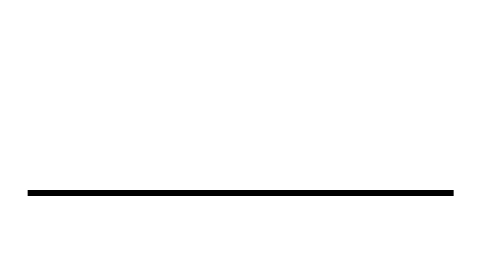
\begin{tikzpicture}
			[line cap=round,line join=round,>=triangle 45,x=1cm,y=1cm]
			\clip(2.3995025373356222,-0.5352732952773178) rectangle (7.8091915039840645,2.099132529626986);
			\draw [line width=2pt,domain=2.3995025373356222:7.8091915039840645] plot(\x,{(-0-0*\x)/2});
		\end{tikzpicture}
		
		\LARGE 2 Geraden\\
		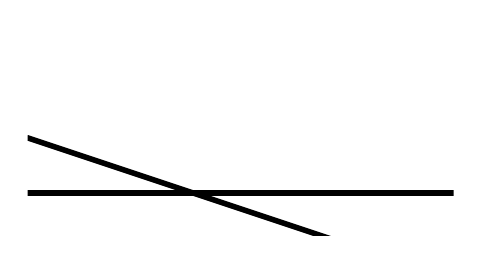
\begin{tikzpicture}
			[line cap=round,line join=round,>=triangle 45,x=1cm,y=1cm]
			\clip(2.3995025373356222,-0.5352732952773178) rectangle (7.8091915039840645,2.099132529626986);
			\draw [line width=2pt,domain=2.3995025373356222:7.8091915039840645] plot(\x,{(-0-0*\x)/2});
			\draw [line width=2pt,domain=2.3995025373356222:7.8091915039840645] plot(\x,{(-2.25--0.5*\x)/-1.5});
		\end{tikzpicture}
		
		\columnbreak
		\LARGE 3 Geraden\\
		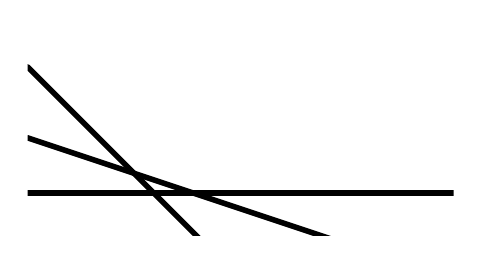
\begin{tikzpicture}
			[line cap=round,line join=round,>=triangle 45,x=1cm,y=1cm]
			\clip(2.3995025373356222,-0.5352732952773178) rectangle (7.8091915039840645,2.099132529626986);
			\draw [line width=2pt,domain=2.3995025373356222:7.8091915039840645] plot(\x,{(-0-0*\x)/2});
			\draw [line width=2pt,domain=2.3995025373356222:7.8091915039840645] plot(\x,{(-2.25--0.5*\x)/-1.5});
			\draw [line width=2pt,domain=2.3995025373356222:7.8091915039840645] plot(\x,{(-4--1*\x)/-1});
		\end{tikzpicture}
		
		\LARGE 4 Geraden\\
		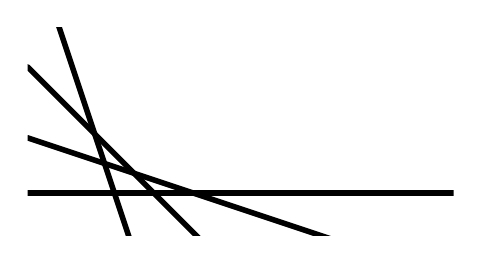
\begin{tikzpicture}
			[line cap=round,line join=round,>=triangle 45,x=1cm,y=1cm]
			\clip(2.3995025373356222,-0.5352732952773178) rectangle (7.8091915039840645,2.099132529626986);
			\draw [line width=2pt,domain=2.3995025373356222:7.8091915039840645] plot(\x,{(-0-0*\x)/2});
			\draw [line width=2pt,domain=2.3995025373356222:7.8091915039840645] plot(\x,{(-2.25--0.5*\x)/-1.5});
			\draw [line width=2pt,domain=2.3995025373356222:7.8091915039840645] plot(\x,{(-4--1*\x)/-1});
			\draw [line width=2pt,domain=2.3995025373356222:7.8091915039840645] plot(\x,{(-5.25--1.5*\x)/-0.5});
		\end{tikzpicture}
		
		\LARGE 5 Geraden\\
		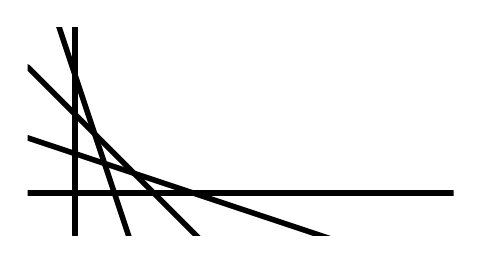
\begin{tikzpicture}
			[line cap=round,line join=round,>=triangle 45,x=1cm,y=1cm]
			\clip(2.3995025373356222,-0.5352732952773178) rectangle (7.8091915039840645,2.099132529626986);
			\draw [line width=2pt,domain=2.3995025373356222:7.8091915039840645] plot(\x,{(-0-0*\x)/2});
			\draw [line width=2pt,domain=2.3995025373356222:7.8091915039840645] plot(\x,{(-2.25--0.5*\x)/-1.5});
			\draw [line width=2pt,domain=2.3995025373356222:7.8091915039840645] plot(\x,{(-4--1*\x)/-1});
			\draw [line width=2pt,domain=2.3995025373356222:7.8091915039840645] plot(\x,{(-5.25--1.5*\x)/-0.5});
			\draw [line width=2pt] (3,-0.5352732952773178) -- (3,2.099132529626986);
		\end{tikzpicture}
		\end{multicols}
		\noindent
		Ausgehend von den Abbildungen können wir folgendes beobachten, hierzu sei n die Anzahl der geraden und F(n) die Anzahl der Begrenzten Flächen:
		\begin{table}[h]
			\centering
			\begin{tabular}{cc}
				n&F(n)\\
				1&0\\
				2&0\\
				3&1\\
				4&3\\
				5&6\\
			\end{tabular}
		\end{table}
	
		\noindent
		Folgende zusammenhänge ergeben sich aus der Tabelle:
		\begin{align*}
			F(1)&=0\\
			F(2)&=0\\
			F(3)&=1\\
			F(4)&=3\\
			F(5)&=6\\
		\end{align*}
		Vermutung: F(n)=F(n-1)+(n-2)\\
		Beispiel: $F(4)=F(3)+2=F(1)+2=1+2=3$\\\\
		Daraus ergibt sich folgendes Rekursionsschema:
		\begin{align*}
			a)\quad\quad\quad\quad F(1)&=0&&&&&&\\
			b)\quad\quad\quad\quad F(2)&=0\\
			c)\quad\quad\quad\quad F(n)&=F(n-1)+(n-2)\\
			d)\quad\quad F(n+1)&=F(n)+(n-1)
		\end{align*}
		
		\noindent
		Hierbei wird n = 1 und n = 2 gesondert betrachtet, da in diesem Bereich für n noch keine begrenzte Fläche geben kann. Optional lässt sich dieses Schema auch in Python übertragen und somit kann man leicht die folgende Tabelle berechnen.
		\lstinputlisting[language=Python]{rekursiv.py}
		\subsection*{b)}
		Im folgenden sind mithilfe des Rekursionschema Werte bis n = 20 für F(n) berechnet:
		\begin{table}[h]
			\begin{tabular}{c|ccccccccccccc}
				n&1&2&3&4&5&6&7&8&9&10&11&12&13\\\hline
				F(n)&0&0&1&3&6&10&15&21&28&36&45&55&66\\
				$\sum\limits_{i=1}^{n}i$&1&3&6&10&15&21&28&36&45&55&66&78&91\\
				$\sum\limits_{i=1}^{n-2}i$&0&0&1&3&6&10&15&21&28&36&45&55&66
			\end{tabular}
		\end{table}
	
		\noindent
		Vermutung: für n > 2\footnote{$\sum\limits_{i=1}^{n}i=\frac{n\cdot(n+1)}{2}$}
		\begin{align*}
			F(n)=\sum\limits_{i=1}^{n-2}i=\frac{(n-2)\cdot((n-2)+1)}{2}
		\end{align*}
		
		\noindent
		Beweis:
		\subsubsection*{Induktionsanfang}
		\begin{tabular}{lcc}
			$F(3)$& $=$ &$\sum\limits_{i=1}^{3-2}i=1\qed$
		\end{tabular}
	
		\subsubsection*{Induktionsvoraussetzung IV}
		für $n=k \in \mathbb{N},\,k \ge 3 \, :$
		\begin{tabular}{lcc}
			$F(k)$ & $=$ & $\sum\limits_{i=1}^{k-2}i$
		\end{tabular}
		\subsubsection*{Induktionsbehauptung}
		für $n=k+1 : F(k+1)=\sum\limits_{i=1}^{k-1}i$
		\subsubsection*{Induktionsbeweis}
		\begin{align*}
			F(k+1) &\overset{d)}{\Rightarrow} F(k)+(k-1)\overset{IV}{\Rightarrow} \textcolor{blue}{\sum\limits_{i=1}^{k-2}i+(k-1)} &&&&&&\\
			\sum\limits_{i=1}^{k-1}i+(k-1) &= 1+2+3+...+k-2+k-1\\
			&=\textcolor{blue}{\sum\limits_{i=1}^{k-2}i+(k-1)}\qed\\
		\end{align*}
		D.h.: für n > 2 gilt: $F(n)=\sum\limits_{i=1}^{n-2}i=\frac{(n-2)\cdot((n-2)+1)}{2}$. Und ist somit die Geschlossene Formel. Dies lässt sich ebenfalls in Python implementieren:
		\lstinputlisting[language=Python]{geschlossene-formel.py}
		
	\section*{3.) „Gärtner Pötschke“}
		\subsection*{a)}
\definecolor{zzwwqq}{rgb}{0.6,0.4,0}
\definecolor{bfffqq}{rgb}{0.7490196078431373,1,0}
\definecolor{ffvvqq}{rgb}{1,0.3333333333333333,0}
\definecolor{ududff}{rgb}{0.30196078431372547,0.30196078431372547,1}
\definecolor{fuqqzz}{rgb}{0.9568627450980393,0,0.6}
\definecolor{qqqqff}{rgb}{0,0,1}
\begin{tikzpicture}[line cap=round,line join=round,>=triangle 45,x=1cm,y=1cm]
	\clip(5.298211392283774,-5.9196311251864255) rectangle (27.239031787601917,4.765091306908912);
	\draw [line width=2pt] (7,4)-- (7,-4);
	\draw [line width=2pt] (15,4)-- (15,-4);
	\draw [line width=2pt] (11,4)-- (11,-4);
	\draw [line width=2pt,color=qqqqff] (15,-3)-- (18,-2);
	\draw [line width=2pt] (19,4)-- (19,-4);
	\draw [line width=2pt,color=qqqqff] (19,-3)-- (22,-2);
	\draw [line width=2pt,color=fuqqzz] (19,-1.964632868187251)-- (16,-1);
	\draw [line width=2pt] (7,-6)-- (7,-14);
	\draw [line width=2pt] (19,-6)-- (19,-14);
	\draw [line width=2pt] (13,-6)-- (13,-14);
	\draw [line width=2pt,color=qqqqff] (7,-13)-- (10,-12);
	\draw [line width=2pt,color=qqqqff] (13,-13)-- (16,-12);
	\draw [line width=2pt,color=qqqqff] (19,-13)-- (22,-12);
	\draw [line width=2pt,color=fuqqzz] (19,-12)-- (16,-11);
	\draw [line width=2pt,color=ffvvqq] (19,-11)-- (22,-10);
	\draw [line width=2pt,color=fuqqzz] (13,-12)-- (10,-11);
	\draw [line width=2pt,color=ffvvqq] (13,-11)-- (16,-10);
	\draw [line width=2pt,color=fuqqzz] (7,-12)-- (4,-11);
	\draw [line width=2pt,color=ffvvqq] (7,-11)-- (10,-10);
	\draw [line width=2pt,color=bfffqq] (13,-10)-- (10,-9);
	\draw [line width=2pt,color=bfffqq] (19,-10)-- (16,-9);
	\draw [line width=2pt,color=zzwwqq] (19,-9)-- (22,-8);
	\draw [line width=2pt] (8.0096263170144,-12.663457894328534)-- (9,-12);
	\draw [line width=2pt] (14.015608565044184,-12.661463811651938)-- (15,-12);
	\draw [line width=2pt] (19.967405948598724,-12.677531350467092)-- (21,-12);
	\draw [line width=2pt] (21.4,-12.2)-- (21.8,-11.6);
	\draw [line width=2pt] (20.5,-12.5)-- (21.8,-12.6);
	\draw [line width=2pt] (14.5,-12.5)-- (15.8,-12.6);
	\draw [line width=2pt] (20.397104372495875,-12.39558690865907)-- (20.6,-12.1);
	\draw [line width=2pt] (11.5,-11.5)-- (11,-11);
	\draw [line width=2pt] (17.5,-11.5)-- (17,-11);
	\draw [line width=2pt] (16.6,-11.2)-- (16.2,-11.3);
	\draw [line width=2pt] (20.2,-10.6)-- (20.8,-10);
	\begin{scriptsize}
		\draw[color=black] (6.876673425235432,-4.976861498825072) node {\LARGE 1. Jahr};
		\draw[color=black] (10.833476824455123,-5.01971466365968) node {\LARGE 2. Jahr}; 
		\draw[color=black] (14.875958707186266,-5.091136605050691) node {\LARGE 3. Jahr};
		\draw[color=black] (18.847018648526398,-5.091136605050691) node {\LARGE 4. Jahr};
	\end{scriptsize}
\end{tikzpicture}

\definecolor{zzwwqq}{rgb}{0.6,0.4,0}
\definecolor{bfffqq}{rgb}{0.7490196078431373,1,0}
\definecolor{ffvvqq}{rgb}{1,0.3333333333333333,0}
\definecolor{ududff}{rgb}{0.30196078431372547,0.30196078431372547,1}
\definecolor{fuqqzz}{rgb}{0.9568627450980393,0,0.6}
\definecolor{qqqqff}{rgb}{0,0,1}
\begin{tikzpicture}[line cap=round,line join=round,>=triangle 45,x=1cm,y=1cm]
	\clip(5.16450638826079,-15.85629532946583) rectangle (26.98113609470271,-5.232051175547066);
	\draw [line width=2pt] (7,4)-- (7,-4);
	\draw [line width=2pt] (15,4)-- (15,-4);
	\draw [line width=2pt] (11,4)-- (11,-4);
	\draw [line width=2pt,color=qqqqff] (15,-3)-- (18,-2);
	\draw [line width=2pt] (19,4)-- (19,-4);
	\draw [line width=2pt,color=qqqqff] (19,-3)-- (22,-2);
	\draw [line width=2pt,color=fuqqzz] (19,-1.964632868187251)-- (16,-1);
	\draw [line width=2pt] (7,-6)-- (7,-14);
	\draw [line width=2pt] (19,-6)-- (19,-14);
	\draw [line width=2pt] (13,-6)-- (13,-14);
	\draw [line width=2pt,color=qqqqff] (7,-13)-- (10,-12);
	\draw [line width=2pt,color=qqqqff] (13,-13)-- (16,-12);
	\draw [line width=2pt,color=qqqqff] (19,-13)-- (22,-12);
	\draw [line width=2pt,color=fuqqzz] (19,-12)-- (16,-11);
	\draw [line width=2pt,color=ffvvqq] (19,-11)-- (22,-10);
	\draw [line width=2pt,color=fuqqzz] (13,-12)-- (10,-11);
	\draw [line width=2pt,color=ffvvqq] (13,-11)-- (16,-10);
	\draw [line width=2pt,color=fuqqzz] (7,-12)-- (4,-11);
	\draw [line width=2pt,color=ffvvqq] (7,-11)-- (10,-10);
	\draw [line width=2pt,color=bfffqq] (13,-10)-- (10,-9);
	\draw [line width=2pt,color=bfffqq] (19,-10)-- (16,-9);
	\draw [line width=2pt,color=zzwwqq] (19,-9)-- (22,-8);
	\draw [line width=2pt] (8.0096263170144,-12.663457894328534)-- (9,-12);
	\draw [line width=2pt] (14.015608565044184,-12.661463811651938)-- (15,-12);
	\draw [line width=2pt] (19.967405948598724,-12.677531350467092)-- (21,-12);
	\draw [line width=2pt] (21.4,-12.2)-- (21.8,-11.6);
	\draw [line width=2pt] (20.5,-12.5)-- (21.8,-12.6);
	\draw [line width=2pt] (14.5,-12.5)-- (15.8,-12.6);
	\draw [line width=2pt] (20.397104372495875,-12.39558690865907)-- (20.6,-12.1);
	\draw [line width=2pt] (11.5,-11.5)-- (11,-11);
	\draw [line width=2pt] (17.5,-11.5)-- (17,-11);
	\draw [line width=2pt] (16.6,-11.2)-- (16.2,-11.3);
	\draw [line width=2pt] (20.2,-10.6)-- (20.8,-10);
	\begin{scriptsize}
		\draw[color=black] (6.893112162744662,-14.762623137150664) node {\LARGE 5. Jahr};
		\draw[color=black] (18.86669213835048,-14.933065556732249) node {\LARGE 7. Jahr};
		\draw[color=black] (12.830189778169611,-14.904658486801985) node {\LARGE 6. Jahr};
	\end{scriptsize}
\end{tikzpicture}

\subsection*{b)}
		Durch abzählen der einzelnen Äste der Abbildung in b) kann man folgendes beobachten:
		\begin{align*}
			Z(1)&=1, & Z(2)&=1, & Z(3)&=2,&&&&&&\\
			Z(4)&=3, & Z(5)&=5, & Z(6)&=8,\\
			Z(7)&=13
		\end{align*}
		Z(n) sei hierbei die Anzahl der Zweige welche nach n Jahren gewachsen sind. Im folgenden sind die Werte für 2 < n < 11 aufgelistet. n=1 und n=2 wurden ignoriert, da es in diesem Zeitraum noch kein Wachstum gibt.
		\begin{table}[h]
			\centering
			\begin{tabular}{l|llllllll}
				n&3&4&5&6&7&8&9&10\\\hline
				Z(n)&\textcolor{blue}{2}&\textcolor{blue}{3}&\textcolor{blue}{5}&\textcolor{blue}{8}&\textcolor{blue}{13}&\textcolor{blue}{21}&\textcolor{blue}{34}&\textcolor{blue}{55}\\
				Z(n-1) &1&2&3&5&8&13&21&34\\
				Z(n-2) &1&1&2&3&5&8&13&21\\
				Z(n-1)+Z(n-2) &\textcolor{blue}{2}&\textcolor{blue}{3}&\textcolor{blue}{5}&\textcolor{blue}{8}&\textcolor{blue}{13}&\textcolor{blue}{21}&\textcolor{blue}{34}&\textcolor{blue}{55}
			\end{tabular}
		\end{table}
	
	\noindent
	Anhand der Tabelle können wir erkennen, dass gilt: $\forall n\in\mathbb{N}\textbackslash\{0,1,2\}$: Z(n) = Z(n-1)+Z(n-2). Also lautet das Rekurionsschema:
	\begin{align*}
		Z(1)&=1\\
		Z(2)&=1\\
		Z(n)&=Z(n-1)+Z(n-2)
	\end{align*}
	Dies ergibt auch Sinn, da ein neuer Zweig zunächst 2 Jahre braucht eh er einen neuen Zweig Produzieren kann. Es muss dementsprechend auf n = 1 und n = 2 gesondert beachtet werden, da in diesem Zeitraum kein neuer Zweig wächst.
\end{document}
